%--------------------------------------
% Create title frame
\titleframe

%--------------------------------------
% Table of contents
\begin{frame}{Overview}
  \setbeamertemplate{section in toc}[sections numbered]
  \tableofcontents[hideallsubsections]
\end{frame}


% Abstract slide
\begin{frame}{Abstract}
    Properly sizing a microgrid is of paramount importance to reach an optimal operation during its entire lifetime. This presentation presents a (stochastic) mixed-integer linear optimization formulation of this sizing problem, emphasizing:
    \begin{itemize}
        \item Generation, converter, and battery storage system degradation
        \item Corresponding necessary reinvestments along the life of the project
        \item Connection costs to the public grid
    \end{itemize}
    
    Considering the evolution of energy and component prices, two scenarios are identified (”optimistic” and ”pessimistic”). 
    
    The resolution of this large optimization problem is facilitated by the use of representative days. 
    
    %The methodology has been applied to the real case of a company already connected to the public grid.
\end{frame}




\section{Optimization objective}

\begin{frame}{What is this section for?}
\begin{itemize}
    \item Investing is always a tradeoff between costs, benefits, value, risk, 
    etc.
    \item The value of money varies with time
    \item Investing requires a financing scheme (e.g. a constant annuity loan)
    \item Besides the technical constraints, it is thus key to determine 
    \begin{itemize}
        \item Which financial objective to optimize (e.g. minimize costs?)
        \item Whether the investment can be funded
        \item How to present results from a financial perspective
    \end{itemize}
\end{itemize}
\end{frame}

\begin{frame}[allowframebreaks]{Net Present Value (NPV)}
  \begin{itemize}
    \item NPV is a metric to determine the \textbf{present value} of future cash flows.
    \item Assesses project profitability.
    \item Accounts for the \textbf{time value of money}.
    \item Considering annual cash flows and a microgrid lifetime of $Y$ years, the $NPV$ can be expressed as:
    \begin{align}
      NPV(c, a) = \sum_{y=1}^{Y} \frac{- I_{y}(c) + R_{y}(c, a) - O_{y}(c, a)}{(1 + d)^{y}}
    \end{align} 
    \item The numerator terms depend on the microgrid sizing decisions $c$ and control decisions $a$ (e will come back to this later), representing annual costs. 
    \item $I$ stands for (re)investment costs $R$ for revenues and $O$ for overall operating costs. 
    \item The present value of the cash flow is obtained by using a discount factor $d$ applied over the microgrid lifetime $Y$. 
    \item Positive NPV $\implies$ Project is expected to generate more value than its costs 
    \begin{itemize}
        \item Example: solar farm, revenues from electricity produced
    \end{itemize}
    \item Negative NPV $\implies$ Project is expected to generate less value than its costs
    \begin{itemize}
        \item Example: microgrid, primary goal is to feed the load
        \item NP is negative because we usually do not account for the value associated with electricity consumption!
        \item even if negative NPV, try to find the least negative value
    \end{itemize}
    \item The NPV becomes positive when the payback period is within the lifetime of the microgrid.
    \item A salvage value may be taken into account.
  \end{itemize}
\end{frame}

\begin{frame}{Capital Expenditure (CAPEX)}
  \begin{itemize}
    \item Funds used to acquire, upgrade, and maintain physical assets.
    \item Examples: property, plants, buildings, technology, equipment.
    \item \textbf{Long-term} investments providing benefits over multiple years.
    \item Distinct from Operating Expenditure (OPEX).
  \end{itemize}
\end{frame}

\begin{frame}{Operating Expenditure (OPEX)}
  \begin{itemize}
    \item Ongoing costs of running a business.
    \item \textbf{Day-to-day} expenses for regular operations.
    \item Examples:
      \begin{itemize}
        \item Salaries
        \item Rent
        \item Utilities
        \item Inventory costs
        \item Marketing expenses
      \end{itemize}
  \end{itemize}
\end{frame}

\begin{frame}{Maintenance}
  \begin{itemize}
    \item Costs associated with keeping assets in good working condition.
    \item Includes:
      \begin{itemize}
        \item Repairs
        \item Regular servicing
        \item Upkeep
      \end{itemize}
    \item Can be CAPEX or OPEX, depending on whether it extends asset life.
  \end{itemize}
\end{frame}

\begin{frame}{Time Value of Money}
  \begin{itemize}
    \item Money available now is worth more than the same amount in the future.
    \item Due to potential earning capacity.
    \item Factors:
      \begin{itemize}
        \item Interest/returns over time.
        \item Inflation eroding purchasing power.
      \end{itemize}
    \item Fundamental principle in finance for informed investment decisions.
  \end{itemize}
\end{frame}

\begin{frame}{NPV Example: Solar Farm Project}
  \begin{itemize}
    \item Project: Construction and operation of a  solar farm.
    \item Initial Investment (CAPEX): €1,000,000
    \item Project lifespan: 5 years
    \item Discount rate: 8\%
  \end{itemize}
\end{frame}

\begin{frame}[allowframebreaks]{Cash Flow Breakdown}
  \begin{itemize}
    \item Year 0:
      \begin{itemize}
        \item CAPEX: -€1,000,000 (Initial Investment)
        \item Funding: €1,000,000 (Loan/Equity)
        \item Net Cash Flow: €0
      \end{itemize}
    \item Year 1:
      \begin{itemize}
        \item Revenue: €300,000
        \item OPEX: -€50,000 (Operational costs)
        \item Maintenance: -€20,000 (Routine servicing)
        \item Net Cash Flow: €230,000
      \end{itemize}
    \item Year 2:
      \begin{itemize}
        \item Revenue: €350,000
        \item OPEX: -€55,000
        \item Maintenance: -€25,000
        \item Net Cash Flow: €270,000
      \end{itemize}
    \item Year 3:
      \begin{itemize}
        \item Revenue: €400,000
        \item OPEX: -€60,000
        \item Maintenance: -€30,000
        \item Net Cash Flow: €310,000
      \end{itemize}
    \item Year 4:
      \begin{itemize}
        \item Revenue: €420,000
        \item OPEX: -€62,000
        \item Maintenance: -€35,000
        \item Net Cash Flow: €323,000
      \end{itemize}
      \item Year 5:
      \begin{itemize}
        \item Revenue: €450,000
        \item OPEX: -€65,000
        \item Maintenance: -€40,000
        \item Residual Value: €100,000 (Sale of equipment)
        \item Net Cash Flow: €445,000
      \end{itemize}
  \end{itemize}
\end{frame}

\begin{frame}{NPV Calculation}
  \begin{itemize}
    \item NPV = $\sum_{t=0}^{n} \frac{CF_t}{(1+r)^t}$
    \item Where:
      \begin{itemize}
        \item $CF_t$ = Cash flow at time t
        \item $r$ = Discount rate (8\% or 0.08)
        \item $n$ = Project lifespan (5 years)
      \end{itemize}
    \item NPV = $-€1,000,000 + \frac{€230,000}{(1.08)^1} + \frac{€270,000}{(1.08)^2} + \frac{€310,000}{(1.08)^3} + \frac{€323,000}{(1.08)^4} + \frac{€445,000}{(1.08)^5}$
    \item NPV $\approx$ €$231,000$
  \end{itemize}
\end{frame}

\begin{frame}{Sensitivity analysis on the discount rate}
\small
\begin{tabular}{l *{5}{S[table-format=3.2E+2]}}
\toprule
Years & Cash flow & \multicolumn{4}{c}{Discount rate} \\
\cmidrule(lr){3-6}
& & {4.00\%} & {8.00\%} & {12.00\%} & {16.00\%} \\
\midrule
0 & -1.00E+06 & -1.00E+06 & -1.00E+06 & -1.00E+06 & -1.00E+06 \\
1 & 2.30E+05 & 2.21E+05 & 2.13E+05 & 2.05E+05 & 1.98E+05 \\
2 & 2.70E+05 & 2.50E+05 & 2.31E+05 & 2.15E+05 & 2.01E+05 \\
3 & 3.10E+05 & 2.76E+05 & 2.46E+05 & 2.21E+05 & 1.99E+05 \\
4 & 3.23E+05 & 2.76E+05 & 2.37E+05 & 2.05E+05 & 1.78E+05 \\
5 & 4.45E+05 & 3.66E+05 & 3.03E+05 & 2.53E+05 & 2.12E+05 \\
\midrule
NPV & 5.78E+05 & 3.88E+05 & 2.31E+05 & 9.90E+04 & -1.22E+04 \\
\bottomrule
\end{tabular}
\end{frame}

\begin{frame}{Conclusion}
  \begin{itemize}
    \item The NPV of the solar farm project is approximately €231,000.
    \item Since the NPV is positive, the project is considered financially viable at an 8\% discount rate.
    \item This example demonstrates how CAPEX, OPEX, maintenance, and funding are factored into NPV calculations.
  \end{itemize}
\end{frame}

\section{Features and constraints}

\begin{frame}[allowframebreaks]{Setup}
We are considering 
\begin{itemize}
    \item multi-year investment $y = 1, 2, \ldots, Y$ (initial investment at year $0$) %TODO
    \item several scenarios $\omega \in \Omega$ with associated probabilities $P(\omega)$ to account for uncertainty %TODO
    \item representative days, so a number $ppy$ of periods per year (same days for all scenarios) to decrease the computational burden %TODO 
\end{itemize}
Hence we are maximizing the \textbf{expected NPV}
\begin{align}
    \max E_{\omega \in \Omega} [NPV] = 
    - I - \sum_{\omega \in \Omega} \left( \sum_{y=1}^{Y}\left(\frac{RI_{y,\omega} + O_{y,\omega} - R_{y,\omega}}{(1 + d)^y}  \right) - \frac{{SV_\omega}}{(1+d)^Y}\right)  \cdot P(\omega)
\end{align}
where $I$ is the initial investment (not subject to uncertainty), and if scenario $\omega$ materializes
\begin{itemize}
    \item $RI_{y,\omega}$ represents a reinvestment in year $y$ 
    \item $O_{y,\omega}$ represents the OPEX in year $y$ 
    \item $R_{y,\omega}$ represents the revenues in year $y$
    \item $SV_{\omega}$ represents the residual value of the assets at the final year $Y$.
\end{itemize}
\end{frame}

\begin{frame}[allowframebreaks]{Sizing problem}
In essence, the sizing problem can be seen as an operational planning problem extended over the lifetime of the project:
\begin{align*}
    \max \quad & E_{\omega \in \Omega} [NPV] \\
    \text{s.t.} \quad & \forall p \in \mathcal{P}, \forall y \in \mathcal{Y}, \forall \omega \in \Omega \\
                 & \quad \text{Planning constraints}  \\
                 & \quad \text{Devices capacity updates and degradation}\\
                 & \quad \text{Definition of CAPEX and OPEX}
\end{align*}
We let device capacities vary (instead of fixed parameters) and account for their CAPEX in the NPV.
We optimize NPV to account for the time value of money, and consider several years to scale OPEX w.r.t. CAPEX.
A variation of the consumption over the years can also be included.

\begin{block}{Example: PV installation sizing (no reinvestment)}
Assuming the PV generation is maximum 10 kW at time $t_1$ for a PV installation of 20 KWp, we constrain the PV power produced at $t_1$ with 
\begin{equation}
    p^{PV}_{t_1} \leq \frac{10}{20} C^{PV} \label{eq:sizing_PV_t1}
\end{equation} with $C^{PV}$ a new variable of the optimization problem, instead of 
$p^{PV}_{t_1} \leq 10$ in a planning problem. We duplicate constraint \eqref{eq:sizing_PV_t1} for all the considered time steps.

$C^{PV}$, multiplied by the unitary cost of PV installation, enters in the NPV estimation.

The problem stays linear, but $C^{PV}$ creates a link between all the time steps.
\end{block}
    
\end{frame}

\begin{frame}[allowframebreaks]{Device capacities}
Let us consider a device $d$ to be sized (e.g., a generator, an inverter, or a battery).

The cost of a device per unit capacity usually decreases as its size increases.
We model this through 
\begin{itemize}
    \item (non-overlapping) capacity intervals $[\underline{\Lambda_{d, c}}, \overline{\Lambda_{d, c}}]$, $c \in \Pi_d$
    \item defining a CAPEX per unit capacity $\pi^{CAPEX}_{d,c}$ parameter such that $$\pi^{CAPEX}_{d,1} > \pi^{CAPEX}_{d,2} > \ldots > \pi^{CAPEX}_{d,|\Pi_d|}$$
    \item defining a binary variable $\beta_{d,c}$ to select one capacity interval.
\end{itemize} 
Then the capacity of device $d$ in the interval $c$ is $\lambda_{d, c}$: 
$$\underline{\Lambda_{d, c}} \cdot \beta_{d, c} \leq \lambda_{d, c}   \leq \overline{\Lambda_{d, c}} \cdot \beta_{d, c}, \ \forall c \in \Pi_d.$$

And the total capacity of device $d$ is 
$\lambda_d   = \sum_{c \in \Pi_d} \lambda_{d,c}$.

We can force the use of at most one interval with 
$\sum_{c \in \Pi_d  } \beta_{d, c} \leq 1.$

Remark: if $|\Pi_d| = 1$, no need to define the variables $\beta_{d,c}$.
\end{frame}



\begin{frame}{Initial investment}
The initial investment cost sums up the microgrid device installation costs and the connection capacity to the public grid.
\begin{equation}
    I = \sum_{d \in \mathcal{D}} \sum_{c \in \Pi_d} \lambda_{d, c} \cdot \pi_{d, c}^{\text{capex}}
    + \mu_{\text{con-cost}}
\end{equation}
With $\mathcal{D} = \mathcal{G} \cup \mathcal{I} \cup \mathcal{B}$.

The public grid connection cost  $\mu_{\text{con-cost}}$ is typically proportional to the power $\kappa^{\text{init}}$ contracted with the system operator, but could also model more complex cost schemes.
\end{frame}


\begin{frame}{Reinvestment, capacity update}
We can apply a similar principle to compute reinvestment in devices, e.g. in device $d$ in year $y$, $\lambda_{d, y}^{\text{ri}}$, and thus to compute the total reinvestment cost in year $y$, $RI_y$. %TODO scenario \omega

We can also consider that some devices have a limited lifetime $T_d$ and account for that in the total capacity at year $y$: 
$$\lambda_{d, y}^{\text{tot}} = \sum_{y'=y-T_d}^y \lambda_{d, y'}^{\text{ri}} + (\lambda_{d} \text{ if } y < T_d)$$

We then use $\lambda_{d, y}^{\text{tot}}$ as a bound in the constraints expressing the constraint on the power of devices in year $y$.
\end{frame}

\begin{frame}[allowframebreaks]{OPEX and revenues}

The costs and revenues related to the exchanges of energy with the grid during year $y$ and for scenario $\omega$ are calculated as follows:
$$\mu^{\text{operation}}_{y, \omega} = \sum_{p=y\cdot ppy}^{(y+1)\cdot ppy} (i^\text{grid}_{p} \cdot \pi_{p, \omega}^{\text{import}}) w_p$$
$$R_{y,\omega} =  \sum_{p=y\cdot ppy}^{(y+1)\cdot ppy} ({e}^\text{grid}_{p} \cdot \pi_{p,\omega}^{\text{export}}) w_p$$
where $ppy$ is the number of periods per year\footnote{See section on representative days.}, $w_p$ the weight associated to period $p$, and $\ensuremath{i}^\text{grid}$ and $\ensuremath{e}^\text{grid}$ the energy imported from and exported to the grid. 

The OPEX can also include 
\begin{itemize}
    \item yearly maintenance costs, e.g. as a percentage of the investment % TODO
    \item yearly public grid connection fees % TODO
    \item peak power costs. % TODO
\end{itemize}
\end{frame}



\begin{frame}{Energy balance}
The \textbf{energy balance} constraint is modeled as follows:
\begin{align}
    \ensuremath{e}^\text{grid}_{p} - \ensuremath{i}^\text{grid}_{p}  &= \sum_{g \in \mathcal{G}}  \theta_{g,p} \Delta_t 
     \\ \notag
    &+ \sum_{b \in \mathcal{B}} (\theta_{b,p}^- - \theta_{b,p}^+) \Delta_t  - \zeta^\text{cons}_p  \Delta_t  \text{~~~~~~~~~~~~} \forall p \in \mathcal{P}
\end{align}
where $\theta_g$ is the renewable power produced, $\theta_b^+$ and $\theta_b^-$ the charging and discharging power of BESS $b$, and $\zeta^\text{cons}$ the overall consumption power.

The import and export are bounded by the contracted power:
\begin{itemize}
    \item  $e^{grid}_p \leq \kappa^{\text{init}} \Delta_t$
    \item  $i^{grid}_p \leq \kappa^{\text{init}} \Delta_t$
\end{itemize}
\end{frame}


\begin{frame}[allowframebreaks]{RES generation rules}
The renewable energy generated must always be below the maximum that can be generated at a time $p$, 
$$\theta_{g, p} \leq \theta^{\text{RES, max}}_{g,p}$$
which is the output per peak kW (per unit) at the considered location times the invested (and reinvested) capacity
$$\theta^{\text{RES, max}}_{g,p} = o^{\text{prod-pu}}_{g,y,p} \cdot \lambda_{g, y}^{\text{tot}} $$
The difference is the curtailed power
$$\theta^{\text{RES-curt}}_{g,p} = \theta^{\text{RES, max}}_{g,p} -  \theta_{g,p}$$
\begin{itemize}
\item All this applies $\forall  g \in \mathcal{G}, \forall  p \in \mathcal{P}$.
\item $o^{\text{prod-pu}}_{g,y,p}$ is the per unit power generated at period $p$ for generator $g$ invested in year $y$ 
\end{itemize}

\begin{block}{Cost of curtailment}
Curtailment leads to an \textbf{opportunity cost}, but it should not be explicitly modeled in the OPEX.    
\end{block}

\end{frame}




\begin{frame}{Hybrid inverter Constraints}
Hybrid inverters connect batteries and PV panels, both on the DC side, to the AC bus of the microgrid.
Therefore, the power generated by the PV together with the power discharged from the BESS must always be less than the usable capacity of the inverters $\lambda_{i, \omega}^{\text{us-cap}}$: 
\begin{align}
    &\sum_{g \in \mathcal{G}}  \theta_{g,p} + \sum_{b \in \mathcal{B}} \theta_{b,p}^{-} \leq \sum_{i \in \mathcal{I}} \lambda_{i,y}^{\text{us-cap}} & \forall  p \in \mathcal{P}
\end{align}
The inverters usable-capacity must be at least half of the PV capacity, although in practice care should be taken so as to avoid excessive voltages and currents on the DC side, depending on the particular inverter selected and PV strings topology:
\begin{align}
    &\sum_{i \in \mathcal{I}} \lambda_{i, y}^{\text{us-cap}} \geq \frac{\sum_{g \in \mathcal{G}}  \lambda_{g} + \sum_{x=2}^{y}
\lambda_{g, x}^{\text{ri}} }{2} &  \forall  y \in \mathcal{Y}
    \label{Constraint:inverter_pv}
\end{align}
\end{frame}

\begin{frame}[allowframebreaks]{Battery}
We assume the batteries can be charged or discharged at a 1C-rate\footnote{They can be fully charged or discharged in 1 hour} 
As the battery capacity fades with time and usage, the charging and discharging power decreases as well. This translates through the use of a new variable $\lambda_{b,p}^\text{us-cap}$ that represents the usable capacity of the BESS at period $p$, which is a function of its degradation level:
\begin{align}
     &\theta_{b,p}^+ \leq  o_b^{+, \text{max}} \cdot \lambda^\text{us-cap}_{b,p} &\forall  b \in \mathcal{B}, \forall  p \in \mathcal{P} \\
     &\theta_{b,p}^- \leq o_b^{-, \text{max}} \cdot \lambda^\text{us-cap}_{b,p} &\forall  b \in \mathcal{B}, \forall  p \in \mathcal{P} 
\end{align}
where $o_b^{+, \text{max}}$ and $o_b^{-, \text{max}}$ are the charge and discharge C-rate of the BESS.


The evolution of the state of charge of the BESS $s_{b,p}$ is therefore governed by the following constraints:
\begin{align}
     &s_{b,p} = s_{b, p-1} + (\theta_{b,p}^+ \cdot \eta_b^+ - \frac{\theta_{b,p}^-}{\eta_b^-}) \Delta_t  \\
     &s_{b,p} \leq \lambda^\text{us-cap}_{b,p}  \\
     &\forall  b \in \mathcal{B}, \forall  p \in \mathcal{P} \notag
\end{align}
where $\eta_b^+$ and $\eta_b^-$ are the charging and discharging efficiencies of the BESS.

The initial state of charge is initialized arbitrarily:
$$s_{b,0} = \frac{\lambda_b}{2}$$

\subsubsection{Battery degradation rule}
The degradation of the usable capacity of the BESS is supposed to be a linear function of the number of cycles. 
One complete charge/discharge cycle is assumed to occur per day. When the maximum number of cycles $nc_{b,\text{max}}$ is reached the BESS is removed from the system and can be replaced by a new one:
\begin{align}
 &\textbf{~if~} nc_{1, b, p} \leq nc_{b,\text{max}}: \textbf{~~~~~~~~~~~~}\forall  b \in \mathcal{B}, \forall  p \in \mathcal{P} \notag\\
     &\textbf{~~~~}\lambda^\text{us-cap}_{b,p} = \left(\frac{us_{b,\text{min}} - 1}{nc_{b,\text{max}}} \cdot nc_{1, b, p} + 1\right)  \lambda_b + \lambda^\text{ri-us-cap}_{b,p} \\
&\textbf{~else~}: \notag \\
    &\textbf{~~~~} \lambda^\text{us-cap}_{b,p} = \lambda^\text{ri-us-cap}_{b,p}
\end{align}
where $nc_{1, b, p}$ is the number of cycles at period $p$ of the initial BESS investment $b$ (at year 1), $us_{b,\text{min}}$ the minimum usable capacity achieved when the number of cycles is maximum, and $\lambda^\text{ri-us-cap}_{b,p}$ the added usable capacity provided by the reinvestments.
The latter is derived by adding up all the reinvested capacities from period 1 to $p$ and computing their degradation using the same procedure as above:
\begin{align}
 &\textbf{~for~} y \in \mathcal{Y}[2, y_p]: \textbf{~~~~~~~~~~~~}\forall  b \in \mathcal{B}, \forall  p \in \mathcal{P} \notag\\ 
 &\textbf{~~~~}\textbf{~if~} nc_{b,y, p} \leq nc_{b,\text{max}}: \notag\\
     &\textbf{~~~~~~~~}\lambda^\text{ri-us-cap}_{b,p} \mathrel{+}= (\frac{us_{b,\text{min}} - 1}{nc_{b,\text{max}}} \cdot nc_{b, y, p} + 1) \cdot \lambda_{b,y}^{\text{ri}}  \\
&\textbf{~~~~~else~}: \notag \\
    &\textbf{~~~~~~~~} \lambda^\text{ri-us-cap}_{b,p} \mathrel{+}= 0
\end{align}
where $y_p$ is the year of period $p$ and $\lambda_{b,y,\omega}^{\text{ri}}$ the reinvestment BESS capacity at year $y$.
\end{frame}



\begin{frame}{Connection Cost}
  \begin{itemize}
    \item Significant upfront investment.
    \item Varies with distance, voltage level, and grid infrastructure.
    \item Impacts project feasibility and profitability.
    \item Can include substation upgrades, line construction, and permitting.
  \end{itemize}
\end{frame}

\begin{frame}{Peak Power consumed or imported}
  \begin{itemize}
    \item Cost of using the grid function of your actual peak injection or consumption.
    \item Usually smaller than grid connection contracted capacity.
  \end{itemize}
\end{frame}

\begin{frame}{Salvage Value Rule (Finite Duration)}
  \begin{itemize}
    \item Residual value of assets at the end of the project's lifespan.
    \item Must consider component degradation and market value.
    \item Requires accurate estimation of asset lifespan and disposal costs.
  \end{itemize}
\end{frame}

\section{Use case}

\begin{frame}[allowframebreaks]{Description}

We are sizing 
\begin{itemize}
    \item a PV installation (panels + inverter)
    \item a storage system (batteries + inverter)
    \item a generator
    \item a connection to the grid
\end{itemize}
We are considering  an investment period of 20 years, one year replicated 20 times (no increase of costs, e.g., fuel costs, etc.)

Data:
\begin{itemize}
    \item One year (2021) of consumption data with 2 EVs, one heat pump, 4 people. Generated with \url{https://github.com/Diffels/ULG_Flex_Residential_Load}. 
    The model estimates the needs of the heat pump from historical temperature records.
    \item One year of PV data from PVgis (2021) for a location in Huy, Belgium (\url{https://re.jrc.ec.europa.eu/pvg_tools/fr/})
    \item Consumption statistics:
    min $51$ W, average $1522$ W, max $12097$ W, energy 13.3 MWh.
    \item 12 representative days obtained with \url{https://github.com/bcornelusse/daysxtractor}
\end{itemize}

\begin{columns}
    \begin{column}{0.5\textwidth}
    Production duration curve \textbf{for $1$ Wp} \\
    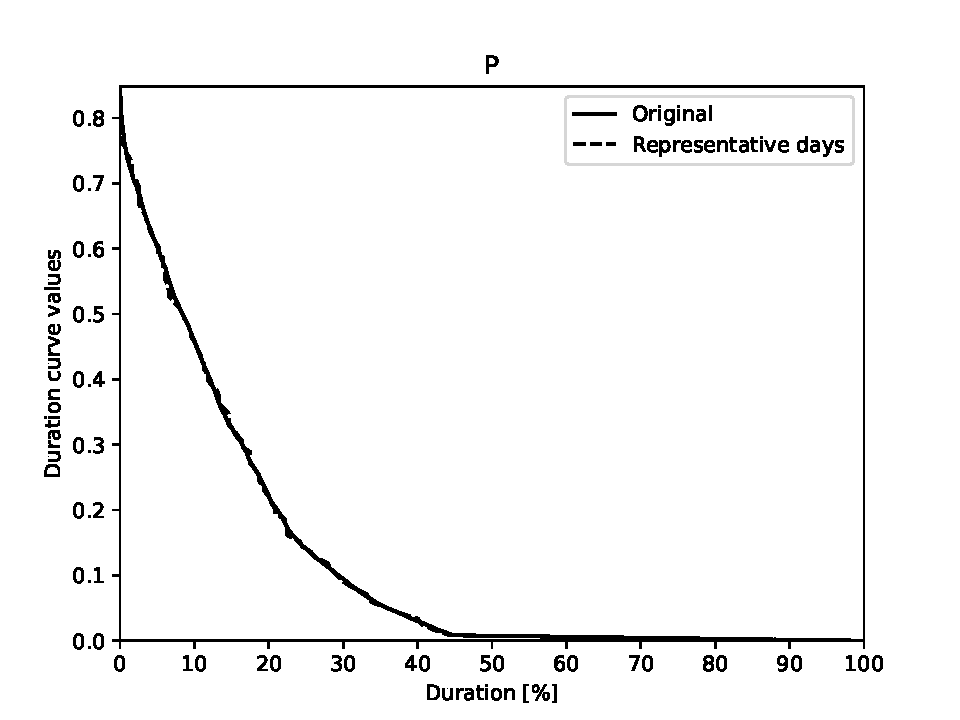
\includegraphics[width=0.9\textwidth]{P.pdf}
    \end{column}
    \begin{column}{0.5\textwidth}
    Load duration curve\\
    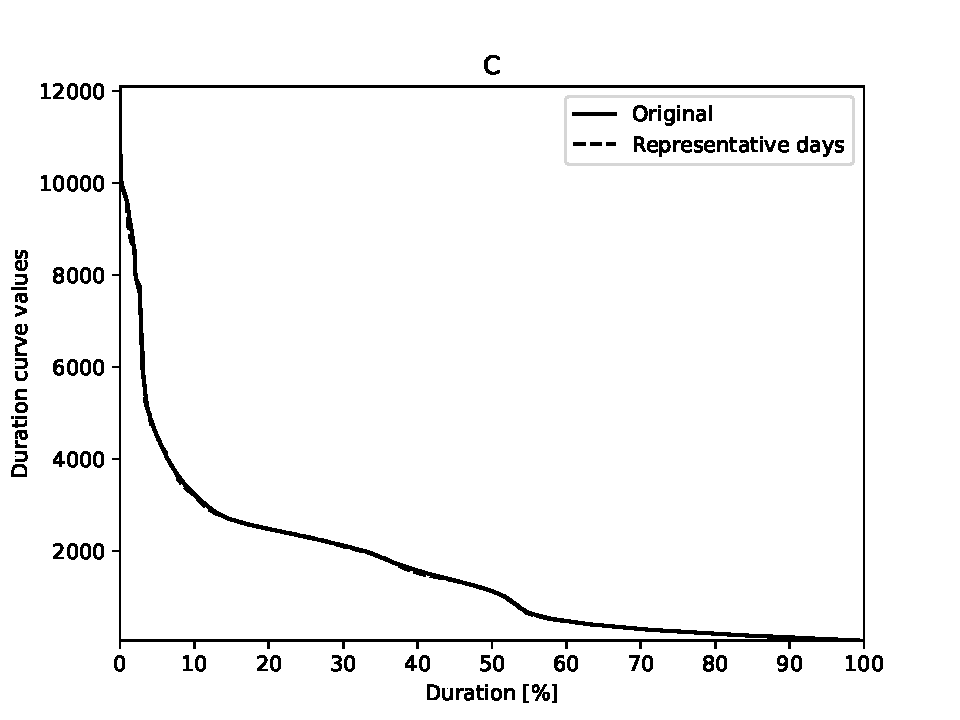
\includegraphics[width=0.9\textwidth]{C.pdf} 
    \end{column}
\end{columns}


\end{frame}

\begin{frame}[allowframebreaks, fragile]{Parameters of the base case}
\lstinputlisting[]{parameters.py}
\end{frame}

\begin{frame}{Results: base case}
\begin{tabular}{lrl}
\hline
 Parameter                           &    Value & Unit   \\
\hline
 NPV (20 years, discount factor 0.0) & -43140.1 & EUR    \\
 CAPEX                               &    13200 & EUR    \\
 Yearly OPEX                         &  1471.26 & EUR    \\
 Grid connection capacity            &        0 & A      \\
 Storage capacity                    &    14.04 & kWh    \\
 Storage inverter capacity           &        6 & kVA    \\
 PV capacity                         &       10 & kWp    \\
 PV inverter capacity                &        7 & kVA    \\
 Genset capacity                     &      5.5 & kVA    \\
\hline
\end{tabular}
\end{frame}

\begin{frame}{Results: exports valorized at 10 cEUR}
\begin{tabular}{lrl}
\hline
 Parameter                           &    Value & Unit   \\
\hline
 NPV (20 years, discount factor 0.0) & -36606.9 & EUR    \\
 CAPEX                               &    11950 & EUR    \\
 Yearly OPEX                         &  1199.37 & EUR    \\
 Grid connection capacity            &       16 & A      \\
 Storage capacity                    &     8.64 & kWh    \\
 Storage inverter capacity           &        4 & kVA    \\
 PV capacity                         &       10 & kWp    \\
 PV inverter capacity                &        8 & kVA    \\
 Genset capacity                     &      5.5 & kVA    \\
\hline
\end{tabular}
\end{frame}

\begin{frame}{Results: exports valorized at 20 cEUR}
\begin{tabular}{lrl}
\hline
 Parameter                           &    Value & Unit   \\
\hline
 NPV (20 years, discount factor 0.0) &   880.39 & EUR    \\
 CAPEX                               &    16080 & EUR    \\
 Yearly OPEX                         & -1010.87 & EUR    \\
 Grid connection capacity            &       64 & A      \\
 Storage capacity                    &        0 & kWh    \\
 Storage inverter capacity           &        0 & kVA    \\
 PV capacity                         &       10 & kWp    \\
 PV inverter capacity                &        8 & kVA    \\
 Genset capacity                     &     16.6 & kVA    \\
\hline
\end{tabular}
\end{frame}

\begin{frame}{Base case with discount factor (0.05)}
\begin{tabular}{lrl}
\hline
 Parameter                            &    Value & Unit   \\
\hline
 NPV (20 years, discount factor 0.05) & -32388.3 & EUR    \\
 CAPEX                                &    11900 & EUR    \\
 Yearly OPEX                          &  1524.27 & EUR    \\
 Grid connection capacity             &        0 & A      \\
 Storage capacity                     &    11.88 & kWh    \\
 Storage inverter capacity            &        5 & kVA    \\
 PV capacity                          &       10 & kWp    \\
 PV inverter capacity                 &        6 & kVA    \\
 Genset capacity                      &      5.5 & kVA    \\
\hline
\end{tabular}
\end{frame}


\begin{frame}{Fuel price increase (0.1 EUR)}
    \begin{tabular}{lrl}
\hline
 Parameter                           &    Value & Unit   \\
\hline
 NPV (20 years, discount factor 0.0) & -55384.3 & EUR    \\
 CAPEX                               &    13700 & EUR    \\
 Yearly OPEX                         &  2084.22 & EUR    \\
 Grid connection capacity            &       16 & A      \\
 Storage capacity                    &    14.04 & kWh    \\
 Storage inverter capacity           &        7 & kVA    \\
 PV capacity                         &       10 & kWp    \\
 PV inverter capacity                &        7 & kVA    \\
 Genset capacity                     &        0 & kVA    \\
\hline
\end{tabular}
\end{frame}


\begin{frame}{Fuel price increase (0.1 EUR) and discount factor (0.05)}
\begin{tabular}{lrl}
\hline
 Parameter                            &    Value & Unit   \\
\hline
 NPV (20 years, discount factor 0.05) & -40786.2 & EUR    \\
 CAPEX                                &    13050 & EUR    \\
 Yearly OPEX                          &  2119.64 & EUR    \\
 Grid connection capacity             &       16 & A      \\
 Storage capacity                     &    12.96 & kWh    \\
 Storage inverter capacity            &        6 & kVA    \\
 PV capacity                          &       10 & kWp    \\
 PV inverter capacity                 &        7 & kVA    \\
 Genset capacity                      &        0 & kVA    \\
\hline
\end{tabular}
\end{frame}

\section{Representative days}
\begin{frame}[allowframebreaks]{Problem statement}
Let's try to give a first definition: 
\begin{block}{Representative days selection: definition 1}
Out of $N_{\text{total}}$ days of data (with a time resolution of $M$ minutes), identify a subset of $N_{\text{repr}}$ days that represent the original data set as well as possible.
\end{block}

This definition is inaccurate because we do not know what a good representation of the original dataset means. Why do we want representative days? 

\begin{itemize}
    \item To solve a problem that takes a long time to solve over $N_{\text{total}}$ days
    \item Overall (including the selection of the days), the time to solve the problem on the $N_{\text{repr}}$ days should be much smaller than the time to solve it on the $N_{\text{total}}$ days.
\end{itemize}

\begin{block}{Representative days selection: definition 2}
Let $\mathcal{P}$ be a problem to be solved over $N_{\text{total}}$ days of data (with a time resolution of $M$ minutes). Identify a subset of $N_{\text{repr}}$ (and their weights)  days such that the solution of $\mathcal{P}$ over the $N_{\text{repr}}$ days has \textbf{the same solution} than the one of the original problem.
\end{block}

Usually, the solution to the original problem is not known, though.
\end{frame}

\begin{frame}[allowframebreaks]{Optimal selection of representative days}
Reference \cite{poncelet2016selecting} proposes to solve the optimization problem 
\begin{subequations}
\begin{align}
\min_{u_d, w_d} \quad & \sum_{c \in \mathcal{C}} \sum_{b \in \mathcal{B}} \left|L_{c, b}-\sum_{d \subset \mathcal{D}} \frac{w_d}{N_{\text {total }}} \cdot A_{c, b, d}\right| \\
\text { s.t. } & \sum_{d \in \mathcal{D}} u_d=N_{\text {repr }}, \\
 & w_d \leq u_d \cdot N_{\text {total }}, \quad \forall d \in \mathcal{D}, \\
 &\sum_{d \in \mathcal{D}} w_d=N_{\text {total }}, \\
 &u_d \in\{0,1\}, \quad w_d \in \mathbb{R}_0^{+}, \quad \forall d \in \mathcal{D} .
\end{align}
\end{subequations}
where 
\begin{itemize}
    \item $u_d=1$ if day $d$ is selected
    \item $w_d$  is the weight associated to day $d$ ($0$ if not  selected)
    \item $\mathcal{C}$ is the set of series considered (e.g., load and PV)
    \item $\mathcal{B}$ is the set of bins used: the duration curves of the series are subdivided into $|\mathcal{B}|$ bins.
    \item the objective minimizes the error between the number of points in the bins in the original data ($L_{c,b}$) and the selected days $A_{c,b,d}$ (weighted by the $w_d$ variables).
\end{itemize}

\newpage

\textit{How can we ensure that the problem $\mathcal{P}$ solved over the $N_{\text {repr }}$ days gives the optimal solution?}     

\begin{itemize}
    \item We cannot really 
    \item We must select enough days (look at the sampling error)
    \item We can estimate costs by simulation on the complete dataset
    \item We can make a study on small problems \cite{dakir2020number}.
\end{itemize}
\end{frame}


\begin{frame}{Decoupling of days}
Since 
\begin{itemize}
    \item the days selected are most of the time not contiguous
    \item the forecasts of load and generation are good for several hours to one day
\end{itemize}
it is common to decouple the days by imposing the equality of the state of the system at the beginning and end of each day day.

The state of charge of storage devices essentially represents the state: 
$$s_d^{init} = s_d^{end}, \forall d \in days.$$
\end{frame}

\begin{frame}[allowframebreaks, fragile]{Bibliography}
  \printbibliography[heading=none]
\end{frame}

\section{Notation}

\begin{frame}{Notation: sets and indices}
\begin{columns}
\begin{column}{0.5\textwidth}    
\begin{itemize}
    \item $b$ Battery index
    \item $c$ Capex index
    \item $d$ Device index
    \item $g$ Generator index
    \item $i$ Inverter index
    \item $p$ Period index
    \item $\nu$ Voltage level index
    \item $\omega$ Scenario index
    \item $y$ Year index
\end{itemize}
\end{column}
\begin{column}{0.5\textwidth}
\begin{itemize}
    \item $\mathcal{B}$ Set of battery energy storage systems
    \item $\Pi$ Set of device capex
    \item $\mathcal{D}$ Set of devices
    \item $\mathcal{G}$ Set of generators
    \item $\mathcal{I}$ Set of inverters
    \item $\mathcal{P}$ Set of periods
    \item $\mathcal{Y}$ Set of years (investment horizon)
    \item $\mathcal{V}$ Set of voltage levels
    \item $\Omega$ Set of scenarios
\end{itemize}
\end{column}

\end{columns}

\end{frame}
\begin{frame}[allowframebreaks]{Notation: parameters}
\begin{itemize}
    \item $d$ Discount factor (\%)
    \item $Y$ Investment horizon (year)
    \item $\pi_{d, c}^{\text{capex}}$ Capex index $c$  of device $d$ (\texteuro/kW - kWh)
    \item $\pi_{d, c}^{\text{maint}}$ maintenance index $c$  of device $d$ (\texteuro/kW - kWh)
    \item $\pi_p^{\text{export}}$ Export electricity price (\texteuro/kWh)
    \item $\pi_p^{\text{import}}$ Import electricity price (\texteuro/kWh)
    \item $\underline{\lambda_{d,c}}$, $\overline{\lambda_{d,c}}$ Lower and upper capacity bound of the capex index $c$ for device $d$
    \item $w_p$ representative day weight of period $p$
    \item $o^{\text{prod-pu}}_g$ Per unit power generated of RES generator $g$ (kW)
    \item $o^{+, \text{max}}$, $o^{-,\text{max}}$ Charge and discharge C-rate of BESS (-)
\end{itemize}
\begin{itemize}
    \item $\zeta^\text{cons}_p$ Overall consumption power (kW)
    \item $\eta_b^+$, $\eta_b^-$ BESS charging and discharging efficiencies (-)
    \item $nc_{b,\text{max}}$ BESS Maximum number of cycle 
    \item $nc_{b,y, p}$ Number of cycle at period $p$ of BESS $b$ installed at year $y$
    \item $us_{b,\text{min}}$ Minimum usable capacity
    \item $\kappa^{\text{init}}$ Actual grid capacity contracted with the distribution system operator
    \item $o^{\text{min}}$, $o^{\text{max}}$ Minimum stable generation and maximum output of diesel generator $g$
\end{itemize}
\end{frame}
\begin{frame}[allowframebreaks]{Notation: variables}
\begin{itemize}
    \item $I$ Initial investment cost (\texteuro) 
    \item $O$ Annual total operational costs (\texteuro) 
    \item $R$ Annual total revenues (\texteuro)
    \item $RI$ Reinvestment costs (\texteuro)
    \item $NPV$ Net present value (\texteuro)
    \item $\lambda$ Device capacity (kW - kWh)
    \item $\ensuremath{i}^\text{grid}$ Energy import from the grid (kWh)
    \item $\ensuremath{e}^\text{grid}$ Energy export to the grid (kWh)
    \item $\theta$ Power generated / exchanged (kW)
    \item $\theta_b^+$; $\theta_b^-$ Battery charging and discharging power (kW)
    \item $\lambda^\text{us-cap}_{b,p}$ BESS usable capacity (kW)
    \item $s_{b,p}$ BESS state of charge (kWh)
    \item $\lambda^\text{ri-us-cap}_{b,p}$ Usable capacity provided by BESS reinvestments
    \item $\lambda_{b,y}^{\text{ri}}$ BESS reinvestment at year $y$
    \item $\peak_{y}$ Peak import at year $y$
    \item $\mu^{\text{op}}_y$ Operating cost related to the energy purchase (\texteuro)
    \item $\mu^{\text{peak}}_y$ Peak penalty cost (\texteuro)
    \item $\mu_{\text{con-cost}}$ Total connection cost (\texteuro)
    \item $\mu_{\text{con-fee}}$ Total connection fee (\texteuro/y) 
    \item $\mu_{\text{con-cost}}^{\text{fix}}$, $\mu_{\text{con-cost}}^{\text{prop}}$ Fixed,  proportional connection cost (\texteuro)
    \item $\mu_{\text{con-fee}}^{\text{fix}}$, $\mu_{\text{con-fee}}^{\text{prop}}$ Fixed, proportional connection fee (\texteuro/$y$)
    \item $\beta$, $k$, $\delta$  Binary variables
\end{itemize}
\end{frame}